\documentclass[12pt,reqno,final,pdftex]{amsart}\usepackage[]{graphicx}\usepackage[]{color}
%% maxwidth is the original width if it is less than linewidth
%% otherwise use linewidth (to make sure the graphics do not exceed the margin)
\makeatletter
\def\maxwidth{ %
  \ifdim\Gin@nat@width>\linewidth
    \linewidth
  \else
    \Gin@nat@width
  \fi
}
\makeatother

\definecolor{fgcolor}{rgb}{0.345, 0.345, 0.345}
\newcommand{\hlnum}[1]{\textcolor[rgb]{0.686,0.059,0.569}{#1}}%
\newcommand{\hlstr}[1]{\textcolor[rgb]{0.192,0.494,0.8}{#1}}%
\newcommand{\hlcom}[1]{\textcolor[rgb]{0.678,0.584,0.686}{\textit{#1}}}%
\newcommand{\hlopt}[1]{\textcolor[rgb]{0,0,0}{#1}}%
\newcommand{\hlstd}[1]{\textcolor[rgb]{0.345,0.345,0.345}{#1}}%
\newcommand{\hlkwa}[1]{\textcolor[rgb]{0.161,0.373,0.58}{\textbf{#1}}}%
\newcommand{\hlkwb}[1]{\textcolor[rgb]{0.69,0.353,0.396}{#1}}%
\newcommand{\hlkwc}[1]{\textcolor[rgb]{0.333,0.667,0.333}{#1}}%
\newcommand{\hlkwd}[1]{\textcolor[rgb]{0.737,0.353,0.396}{\textbf{#1}}}%

\usepackage{framed}
\makeatletter
\newenvironment{kframe}{%
 \def\at@end@of@kframe{}%
 \ifinner\ifhmode%
  \def\at@end@of@kframe{\end{minipage}}%
  \begin{minipage}{\columnwidth}%
 \fi\fi%
 \def\FrameCommand##1{\hskip\@totalleftmargin \hskip-\fboxsep
 \colorbox{shadecolor}{##1}\hskip-\fboxsep
     % There is no \\@totalrightmargin, so:
     \hskip-\linewidth \hskip-\@totalleftmargin \hskip\columnwidth}%
 \MakeFramed {\advance\hsize-\width
   \@totalleftmargin\z@ \linewidth\hsize
   \@setminipage}}%
 {\par\unskip\endMakeFramed%
 \at@end@of@kframe}
\makeatother

\definecolor{shadecolor}{rgb}{.97, .97, .97}
\definecolor{messagecolor}{rgb}{0, 0, 0}
\definecolor{warningcolor}{rgb}{1, 0, 1}
\definecolor{errorcolor}{rgb}{1, 0, 0}
\newenvironment{knitrout}{}{} % an empty environment to be redefined in TeX

\usepackage{alltt}
%% DO NOT DELETE OR CHANGE THE FOLLOWING TWO LINES!
%% $Revision$
%% $Date$
\usepackage[round,sort,elide]{natbib}
\usepackage{graphicx}
\usepackage{times}
\usepackage{rotating}
\usepackage{subfig}
\usepackage{color}
\newcommand{\aak}[1]{\textcolor{cyan}{#1}}
\newcommand{\mab}[1]{\textcolor{red}{#1}}
\newcommand{\cec}[1]{\textcolor{blue}{#1}}

\setlength{\textwidth}{6.25in}
\setlength{\textheight}{8.75in}
\setlength{\evensidemargin}{0in}
\setlength{\oddsidemargin}{0in}
\setlength{\topmargin}{-.35in}
\setlength{\parskip}{.1in}
\setlength{\parindent}{0.3in}

%% cleveref must be last loaded package
\usepackage[sort&compress]{cleveref}
\newcommand{\crefrangeconjunction}{--}
\crefname{figure}{Fig.}{Figs.}
\Crefname{figure}{Fig.}{Figs.}
\crefname{table}{Table}{Tables}
\Crefname{table}{Tab.}{Tables}
\crefname{equation}{Eq.}{Eqs.}
\Crefname{equation}{Eq.}{Eqs.}
\crefname{appendix}{Appendix}{Appendices}
\Crefname{appendix}{Appendix}{Appendices}
\creflabelformat{equation}{#2#1#3}

\theoremstyle{plain}
\newtheorem{thm}{Theorem}
\newtheorem{corol}[thm]{Corollary}
\newtheorem{prop}[thm]{Proposition}
\newtheorem{lemma}[thm]{Lemma}
\newtheorem{defn}[thm]{Definition}
\newtheorem{hyp}[thm]{Hypothesis}
\newtheorem{example}[thm]{Example}
\newtheorem{conj}[thm]{Conjecture}
\newtheorem{algorithm}[thm]{Algorithm}
\newtheorem{remark}{Remark}
\renewcommand\thethm{\arabic{thm}}
\renewcommand{\theremark}{}

\numberwithin{equation}{part}
\renewcommand\theequation{\arabic{equation}}
\renewcommand\thesection{\arabic{section}}
\renewcommand\thesubsection{\thesection.\arabic{subsection}}
\renewcommand\thefigure{\arabic{figure}}
\renewcommand\thetable{\arabic{table}}
\renewcommand\thefootnote{\arabic{footnote}}

\newcommand\scinot[2]{$#1 \times 10^{#2}$}
\newcommand{\code}[1]{\texttt{#1}}
\newcommand{\pkg}[1]{\textsf{#1}}
\newcommand{\dlta}[1]{{\Delta}{#1}}
\newcommand{\Prob}[1]{\mathbb{P}\left[#1\right]}
\newcommand{\Expect}[1]{\mathbb{E}\left[#1\right]}
\newcommand{\Var}[1]{\mathrm{Var}\left[#1\right]}
\newcommand{\dd}[1]{\mathrm{d}{#1}}
\newcommand{\citetpos}[1]{\citeauthor{#1}'s \citeyearpar{#1}}
\IfFileExists{upquote.sty}{\usepackage{upquote}}{}
\begin{document}



\section*{DEB fitting with dynamic algae}
To begin, I am going to do some simulation/recovery experiments with a DEB model with a dynamically varying resource.
The model I am going to start with is the following:
\begin{align}
\frac{dF}{dt} &= -I_{max} \frac{F}{f_h+F} L_{obs}^g \\
\frac{dE}{dt} &= \rho \epsilon V I_{max} \frac{F}{f_h+F} L_{obs}^g - p_C, \\
\frac{dW}{dt} &= \kappa~p_C - k_M~W, \\
\frac{dR}{dt} &= \frac{(1-\kappa)~p_C}{E_R}, \\
p_C &= E \left(\frac{\frac{v}{L} + k_m}{1+\frac{\kappa E}{W}}\right).
\end{align}
This model makes the simplifying assumption that the algae are not reproducing.
I will deal with that problem later..
However, I will assume that an amount of food $F_{a}$ is added every day, and that every fifth day the food is reset to $F_{a}$, corresponding to the transfer of the animal to a clean beaker.
The parameters of the feeding model are specified by the best-fitting model above.
However, this model tracks the dynamics of the concentration of algae in cells/ml; to get the total amount of carbon assimilated by the daphnid, I simply multiply the ingestion by $\rho$, the assimilation efficiency, $\epsilon$, the carbon content per cell, and $V$, the total volume of the container.

I performed a quick simulation study to see how well the model was able to recover the parameter estimates.
I simulated a dataset assuming $I_{max}=22500$, $f_h=10000$, $g=1.45$, $\rho=0.1$, $\epsilon = 44.5\times10^{-9}$, $V=30$, $\kappa=0.3$, $k_m=0.15$, $E_R=0.00151$, and $v=10$.
To generate observation error, I assumed that length observations were normally distributed with mean equal to the simulated length and standard deviation equal to $\sigma_L=0.1$.
I assumed the observation of neonates was Poisson distributed, so the mean and standard deviation are equal and given by the true egg production.
Thus, there were no parameters to estimate for the error in the observation of reproduction.
I simulated a dataset that was similar in struture to the true dataset I will try fit later.
That is, I simulated 10 observations of length and cumulative egg production at ages 5, 10, 12, 15, 18, 25, 30, and 35.
This essentially assumes that I have observed the growth and reproduction of 10 individuals that have identical parameters and differ from one another only because observation is not perfect.
This is a strong assumption - in reality I should simulate a model with demographic stochasticity (at the very least) and almost certainly with extrademographic stochasticity, given the stochasticity inherent in the feeding protocol.

Including such sources of stochasticity would make the fitting much more complicated.
When there is only observation error, I am performing \emph{trajectory matching}.
That is, given a set of observations $y_t$ at timepoints $t \in (1,\ldots,T)$ and a model with parameters $\theta$ that predicts states $x_t$, the measurement error model gives a way of calculating the probability of $y_t$, given the true system state of $x_t$, as $P(y_t | x_t, \theta)$.
Then the likelihood of the parameter set $\theta$ (and thus the model itself) can be written as
\begin{equation}
\mathcal{L}(\theta) = P(y_{1:T}|\theta) = \prod_t P(y_t | x_t, \theta).
\end{equation}
I simply need to find the set of parameters $\theta$ that maximize this likelihood (or, in practice, minimize its negative logarithm).
This is fairly straightforward.
If, however, I assume that there is stochasticity either due to demographic or extrademographic processes, the likelihood maximization becomes much more complicated.
The reason is because a single set of parameters $\theta$ can now generate many different $x_t$ trajectories.
To evaluate the likelihood of a single set of parameters, it is necessary to integrate over all of the \emph{possible} trajectories that could have been produced.
That is, we now need to maximize the likelihood function
\begin{equation}
\mathcal{L}(\theta) = P(y_{1:T}|\theta) = \sum_{x_1} \cdots \sum_{x_T} \prod_t P(y_t | x_t, \theta) P(x_t | x_{1:t-1},\theta).
\end{equation}
where we have the additional term that computes the likelihood of observing $x_t$, given the trajectory from time 1 to time $t-1$.
Maximizing this function requires Monte Carlo methods to carry out the necessary high dimensional integration.
I don't want to deal with that yet (and possibly not ever!), so I will focus only on trajectory matching right now.

I attempted to estimate only $\kappa$, $k_m$, $E_R$, $v$, and $\sigma_L$.
You can see from Fig. \ref{fig:dyn-food-hist} that, with the exception of $v$, the parameters were actually fairly well estimated.
Moreover, if you actually look at the log-likelihoods of the best-fitting parameter set and the true parameter set, you find that the best-fitting parameters are actually better than the truth, with the best-fit parameters having a log-likelihood of -90.5 compared to a negative log-likelihood of -91.2 (this is a not-uncommon finding, and it strongly suggests that the fitting algorithm really is honing in).

\begin{knitrout}\scriptsize
\definecolor{shadecolor}{rgb}{0.969, 0.969, 0.969}\color{fgcolor}\begin{figure}

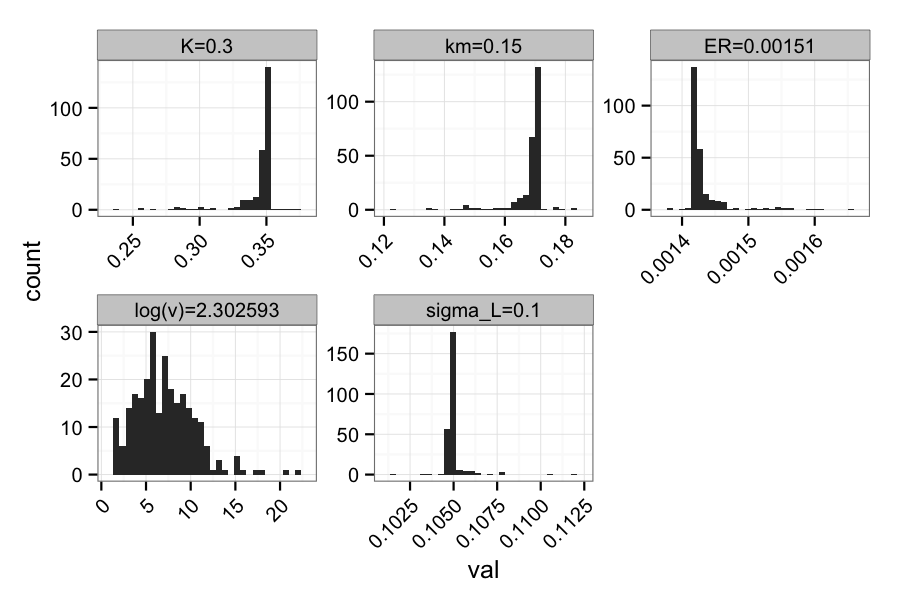
\includegraphics[width=\linewidth]{figure/dyn-food-hist-1} \hfill{}

\caption[Parameter estimates when food is dynamic]{Parameter estimates when food is dynamic.}\label{fig:dyn-food-hist}
\end{figure}


\end{knitrout}

If you construct the profile likelihood for $v$ by fixing it at different values and fitting all of the other parameters, you can see that many values of $v$ are equally supported by the data (Fig. \ref{fig:dyn-food-prof-lik-v}), and the other parameter estimates are closer to the truth when $v$ is fixed at smaller values.
\begin{knitrout}\scriptsize
\definecolor{shadecolor}{rgb}{0.969, 0.969, 0.969}\color{fgcolor}\begin{figure}

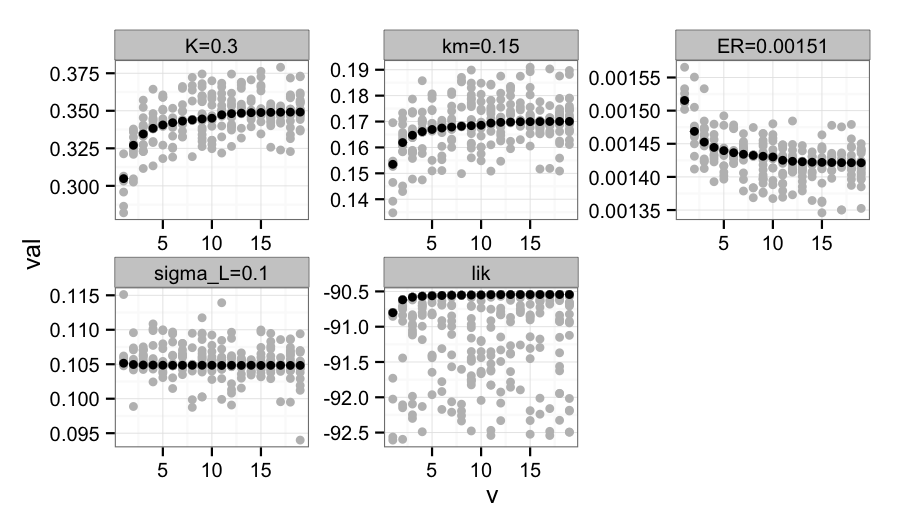
\includegraphics[width=\linewidth]{figure/dyn-food-prof-lik-v-1} \hfill{}

\caption[DEB parameters under dynamic food, when ]{DEB parameters under dynamic food, when $v$ is fixed at different values.}\label{fig:dyn-food-prof-lik-v}
\end{figure}


\end{knitrout}

I am also interested in whether $f_h$ can be estimated on the basis of growth and reproduction data.
For this simulation-recovery experiment, I again fixed $v$ at different values and then attempted to estimate $f_h$ along with $\kappa$, $k_m$, $E_R$, and $\sigma_L$.
During the fitting, as different values of $f_h$ were investigated, the values of $I_{max}$ and $g$ were set at the values that maximized the likelihood based on fitting the feeding data - this should deal with the fact that many different values of $f_h$ could fit the feeding data equally well.
For any fixed value of $v$, a large range of $f_h$ values are nearly equally well-supported, and the value of all of the other DEB parameters scales with the value of $f_h$ (Fig. \ref{fig:dyn-food-pairwise}).
There is a peak in the likelihood surface at intermediate $f_h$, which is encouraging, as this peak is actually fairly close to the true value of $f_h$.
The best-fit parameter value is shown by the blue point, and the true value is shown by the red point, so, again, all of the parameters are slightly mis-estimated, but this is probably to be expected.
I still have good evidence that the model can be recovered reasonably well, which is, in and of itself, pretty encouraging.

\begin{knitrout}\scriptsize
\definecolor{shadecolor}{rgb}{0.969, 0.969, 0.969}\color{fgcolor}\begin{figure}

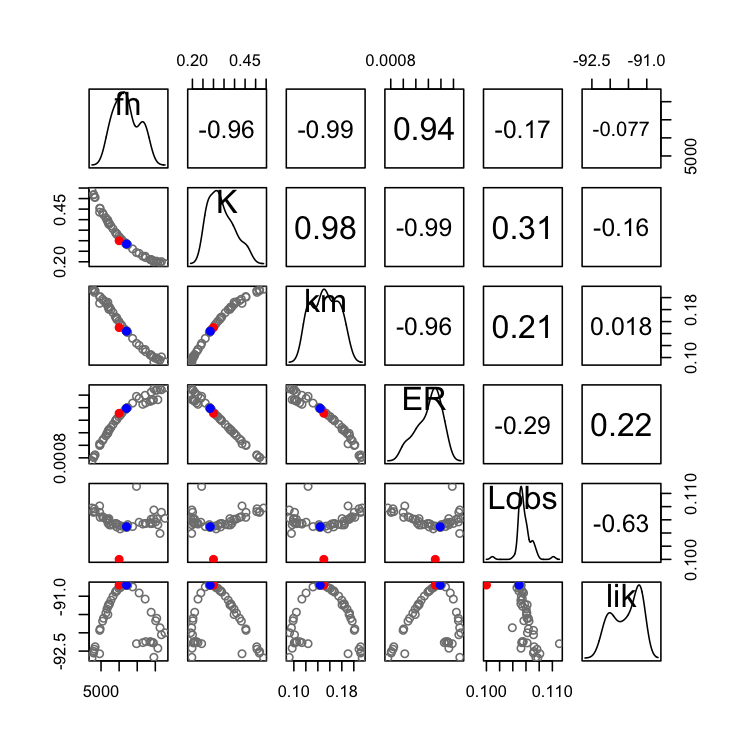
\includegraphics[width=\linewidth]{figure/dyn-food-pairwise-1} \hfill{}

\caption[Pairwise scatterplot of estimates of ]{Pairwise scatterplot of estimates of $f_h$ and DEB parameters when $v=10$.}\label{fig:dyn-food-pairwise}
\end{figure}


\end{knitrout}

We can also look at only the best-fitting parameter set across a range of $v$ values to see how the best-fitting estimate of $f_h$ (and hence the other parameters) depends on the fixed value of $v$.
Fig. \ref{fig:dyn-food-fh-est-profile-v} shows all of the parameter estimates within 2 log-likelihood units of the maximum, for different fixed values of $v$.
Again, you can see that a large number of $f_h$ values are reasonably well supported, driving a lot of variation in the other estimates.
Still, however, the estimate of $f_h$ is reasonably good, and smaller values of $v$, though they have lower likelihoods, produce better estimates of the DEB parameters (though worse estimates of $f_h$).

\begin{knitrout}\scriptsize
\definecolor{shadecolor}{rgb}{0.969, 0.969, 0.969}\color{fgcolor}\begin{figure}

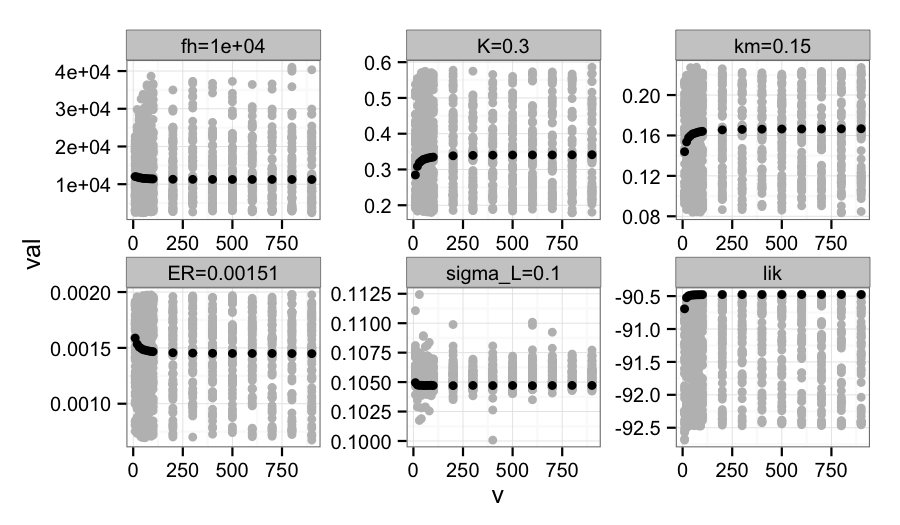
\includegraphics[width=\linewidth]{figure/dyn-food-fh-est-profile-v-1} \hfill{}

\caption[Estimates of ]{Estimates of $f_h$ and the DEB parmaeters as $v$ is varied.}\label{fig:dyn-food-fh-est-profile-v}
\end{figure}


\end{knitrout}

\clearpage

I have left aside one fitting problem till now: estimating $\rho$.
I have the distinct feeling that assimilation efficiency will be almost impossible to estimate, as there will be ways to jigger the other parameters to get equally good fits with almost any value of $\rho$.
To investigate this, I fixed the value of $v=100$ and tried to estimate the DEB parameters, along with $\rho$ and $f_h$.
Fig. \ref{fig:estimating-rho} shows these difficulties.
The estimates of $\rho$ range between 0.2 and 1, with the majority of estimates being very near 1.
There are also clear correlationshp between the estimates of $\rho$ and $\kappa$ and $E_R$, in particular.
These make sense: as assimilation efficiency increases, $\kappa$ must decrease to keep size reasonable; but as $\kappa$ decreases, the cost of reproduction must increase to keep the total egg production reasonable.
The estimates of  $f_h$, $k_m$, and $\sigma_L$ are all still centered near their true values, with likelihood peaks at those values.

\begin{knitrout}\scriptsize
\definecolor{shadecolor}{rgb}{0.969, 0.969, 0.969}\color{fgcolor}\begin{figure}

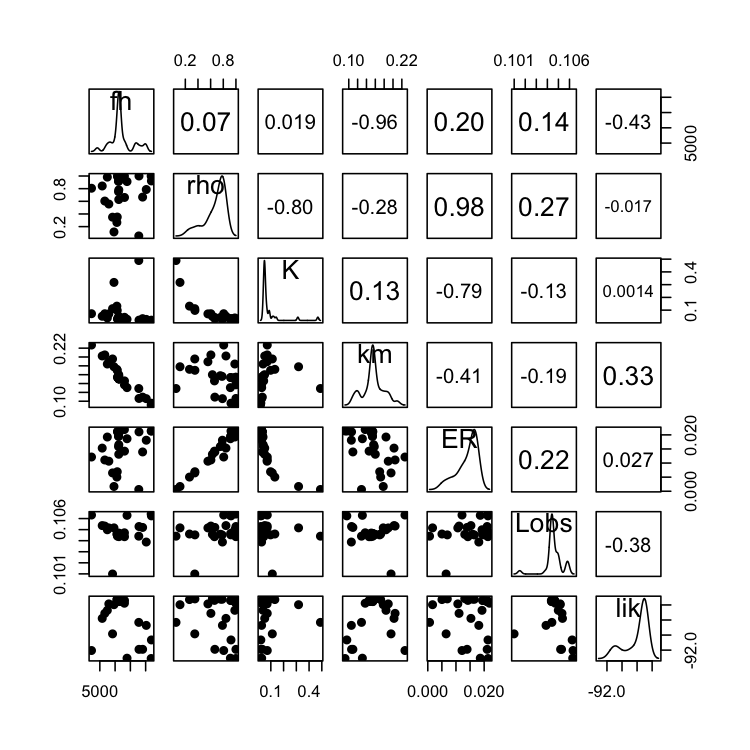
\includegraphics[width=\linewidth]{figure/estimating-rho-1} \hfill{}

\caption[Scatterplot of parameter estimates when ]{Scatterplot of parameter estimates when $
ho$ is estimated along with $f_h$ and the other DEB parameters. $v$ was fixed at $v=100$ for this estimation.}\label{fig:estimating-rho}
\end{figure}


\end{knitrout}

To further determine how big of a problem estimating $\rho$ is, I did the same kind of profile likelihood calculation, fixing $\rho$ at values between 0.1 and 0.9 and estimating all of the other parameters.
You can see that the fixed value of $\rho$ drives the estimates of $\kappa$ and $E_R$, as before, and that $f_h$, $k_m$, $\sigma_L$ are all reasonably estimated (Fig. \ref{fig:rho-profile}).
More problematically, however, the likelihood increases with increasing values of $\rho$, even though the true value of $\rho$ was 0.1.
This certainly supports my supposition that $\rho$ is very hard to estimate.

\begin{knitrout}\scriptsize
\definecolor{shadecolor}{rgb}{0.969, 0.969, 0.969}\color{fgcolor}\begin{figure}

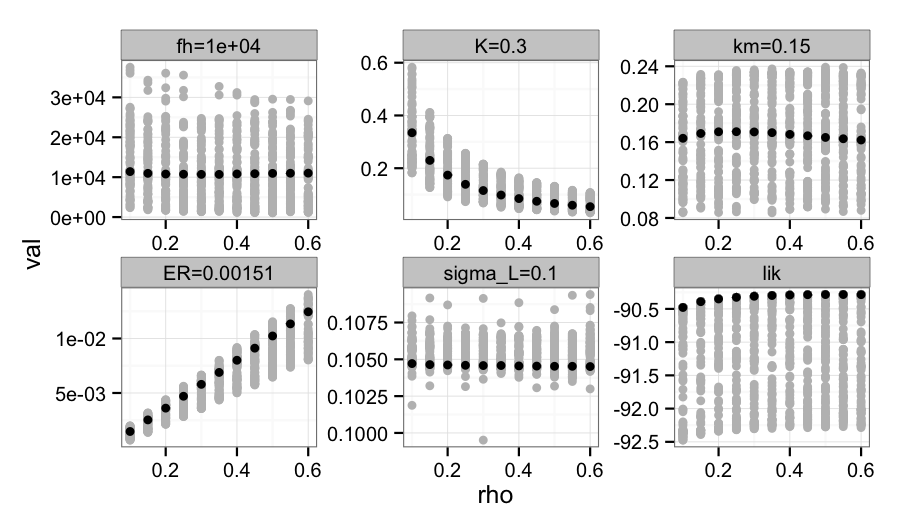
\includegraphics[width=\linewidth]{figure/rho-profile-1} \hfill{}

\caption[Estimates of ]{Estimates of $f_h$ and DEB parameters for different fixed values of $
ho$. For these $v$ was fixed at $v=100$ since there is no evidence so far that the value of that parameter affects the other parameter estimates.}\label{fig:rho-profile}
\end{figure}


\end{knitrout}

However, the strong linear relationship between the fixed value of $\rho$ and the maximum likelihood estimate of $E_R$ suggests a way to estimate $\rho$:
if the value of $E_R$ could be fixed, rather than estimated, that should much more greatly constrain the value of $\rho$.
And, fortunately, $E_R$ is a parameter that is likely plausibly estimated based on the size (and thus, carbon content) of a newborn daphnid.
With that in mind, I redid the fitting, assuming that $E_R = 1.51\times10^{-3}$, the true value in the simulated dataset.
Fig. \ref{fig:est-rho-fix-ER} shows pairwise scatterplots of the parameter estimates when $E_R$ is fixed at its true value and $v$ is fixed at 1000.
You can see from the density plots along the diagonal that the bulk of the estimates are, indeed, close to the true values ($f_h=10000$, $\rho=0.1$, $\kappa=0.3$, $k_m=0.15$, $\sigma_L=0.1$), and that these values correspond to peaks on the likelihood surface.
\begin{knitrout}\scriptsize
\definecolor{shadecolor}{rgb}{0.969, 0.969, 0.969}\color{fgcolor}\begin{figure}

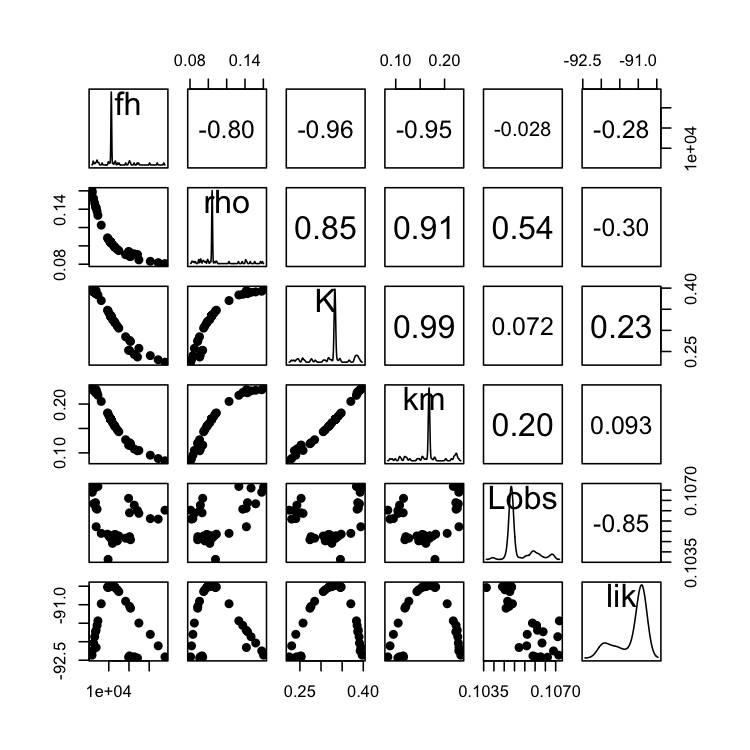
\includegraphics[width=\linewidth]{figure/est-rho-fix-ER-1} \hfill{}

\caption[Parameter estimates when ]{Parameter estimates when $E_R$ is fixed at the true value and $v=1000$.}\label{fig:est-rho-fix-ER}
\end{figure}


\end{knitrout}

If you look across a range of fixed $v$ values, the best-fitting parameter estimates also seem to hone right in on parameter estimates that are close to the true values (Fig. \ref{fig:profile-lik-v-estimating-rho}; the black points show the parameter estimate with highest likelihood).
In particular, the estimates of $\rho$ are quite good.

\begin{knitrout}\scriptsize
\definecolor{shadecolor}{rgb}{0.969, 0.969, 0.969}\color{fgcolor}\begin{figure}

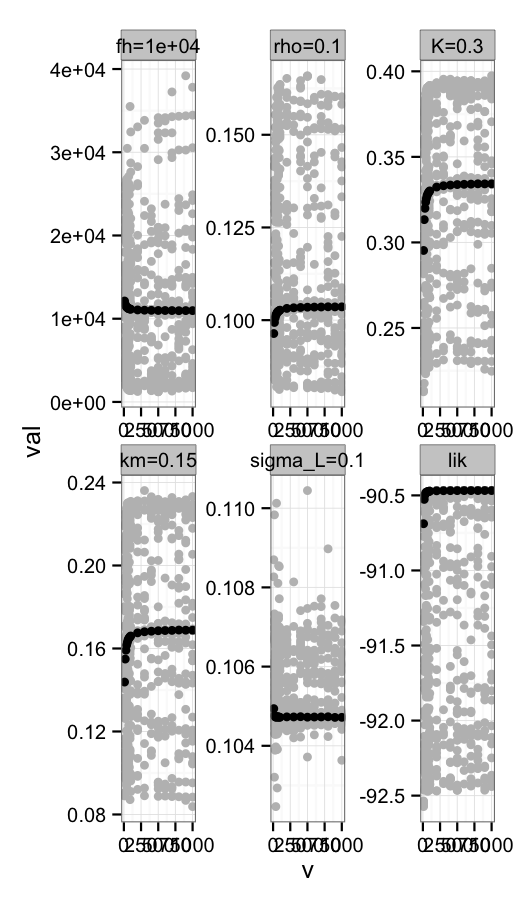
\includegraphics[width=\linewidth]{figure/profile-lik-v-estimating-rho-1} \hfill{}

\caption[Estimates of DEB parameters across a range of ]{Estimates of DEB parameters across a range of $v$ values, when $E_R$ is fixed at its true value.}\label{fig:profile-lik-v-estimating-rho}
\end{figure}


\end{knitrout}

\clearpage

Okay, all of the preceding has been based on fitting a single dataset, and hence a single parameter set.
The last thing to do before moving on to deal with the real data is to simulate datasets with a much wider range of parameter values and attempt to fit those datasets as well.
For this, I generated 20 simulated datasets.
There were some constraints on the parameters and the simulated datasets, to ensure they were somewhat biologically realistic for \emph{Daphnia}.
In particular, all of the parameters had to be positive and $\rho$ and $\kappa$ had to be between 0.1 and 0.9.
I also only accepted parameter sets that produced simulated data such that the observed length at day 5 was less than 2 mm and the observed egg production was 0; moreover, the length at day 35 had to be between 0.5 and 4mm and the egg production at day 35 had to between 5 and 200 eggs.
Finally, some growth had to be observable in the data (a linear regression of length against time had to have a significantly positive slope).
These are fairly tame restrictions; Fig. \ref{fig:sim-datasets} shows smoothed fits of the growth and reproduction data through time to show the variability in growth and reproduction trajectories across the datasets.

\begin{knitrout}\scriptsize
\definecolor{shadecolor}{rgb}{0.969, 0.969, 0.969}\color{fgcolor}\begin{figure}

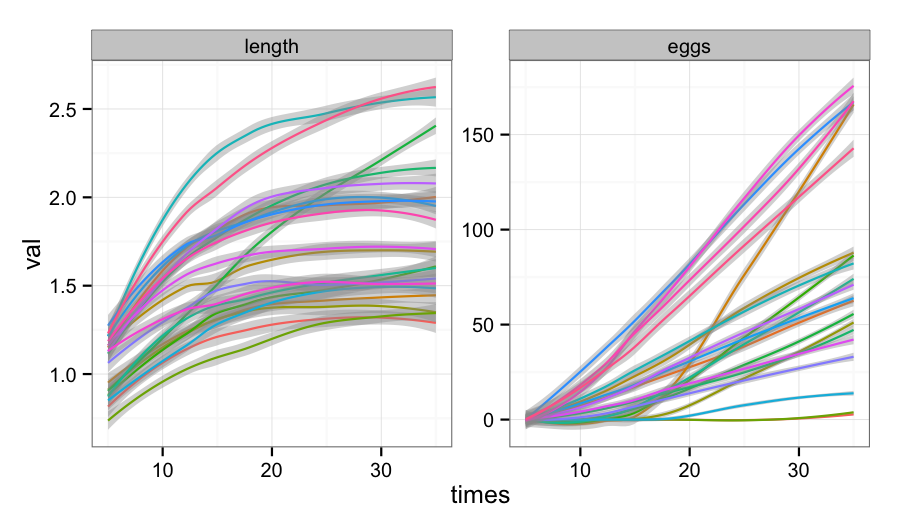
\includegraphics[width=\linewidth]{figure/sim-datasets-1} \hfill{}

\caption[Growth and reproduction trajectories across the 20 simulated datasets]{Growth and reproduction trajectories across the 20 simulated datasets. What is shown is not the raw data, but a smoothed fit of that data. This cleans up the figures but still shows the variability among datasets.}\label{fig:sim-datasets}
\end{figure}


\end{knitrout}

Fig. \ref{fig:mult-datasets-fitting} plots the results of the fitting.
For every parameter set (1-20), I plot all of the parameter estimates that were within 2 log-likelihood units of the best-fitting parameter set.
The parameter set with highest likelihood is shown in black.
The true parameter value is shown in red.
You can see that the overall message here is really encouraging - the best-fitting parameter estimates are typically quite close to the true values.
The exception is certainly with a few of the estimates of $f_h$ (e.g., datasets 10 and 12).
Some datasets also elicited a lot more variability in the parameter estimates that were near the highest likelihood (e.g., dataset 18).
The estimates of $k_m$ were the most variable

\begin{knitrout}\scriptsize
\definecolor{shadecolor}{rgb}{0.969, 0.969, 0.969}\color{fgcolor}\begin{figure}

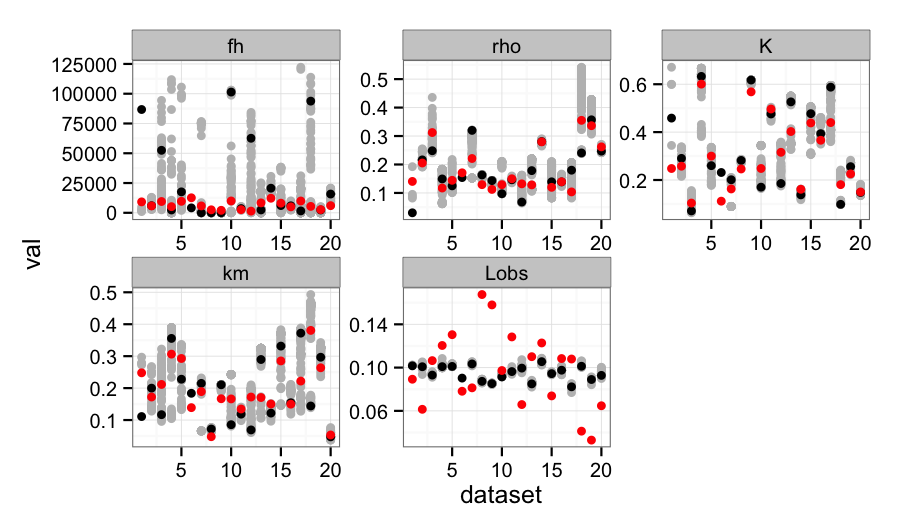
\includegraphics[width=\linewidth]{figure/mult-datasets-fitting-1} \hfill{}

\caption[Parameter estimates across 20 different parameter sets]{Parameter estimates across 20 different parameter sets. The black point shows the best-fitting parameter estimate. The grey points are parameter estimates within 2 log-likelihood units of the best. The red point is the true parameter value. For these fits, $v$ was fixed at 100.}\label{fig:mult-datasets-fitting}
\end{figure}


\end{knitrout}

An examination of the plots of the likelihood against the parameter estimates can help to understand when the parameter estimates were close the true parameter values.
Fig. \ref{fig:lik-against-ests-1} shows some likelihood surfaces when the parameter estimates were quite close to the truth (similar surfaces were revealed for other datasets that were well-estimated (datasets 3, 15, 16, 17, and 20).
Here you can see a single, well-defined likelihood peak.
In this case, the best-fitting parameter estimate (shown by the vertical green line) is quite close to the true parameter estimate (shown by the vertical red line).

\begin{knitrout}\scriptsize
\definecolor{shadecolor}{rgb}{0.969, 0.969, 0.969}\color{fgcolor}\begin{figure}

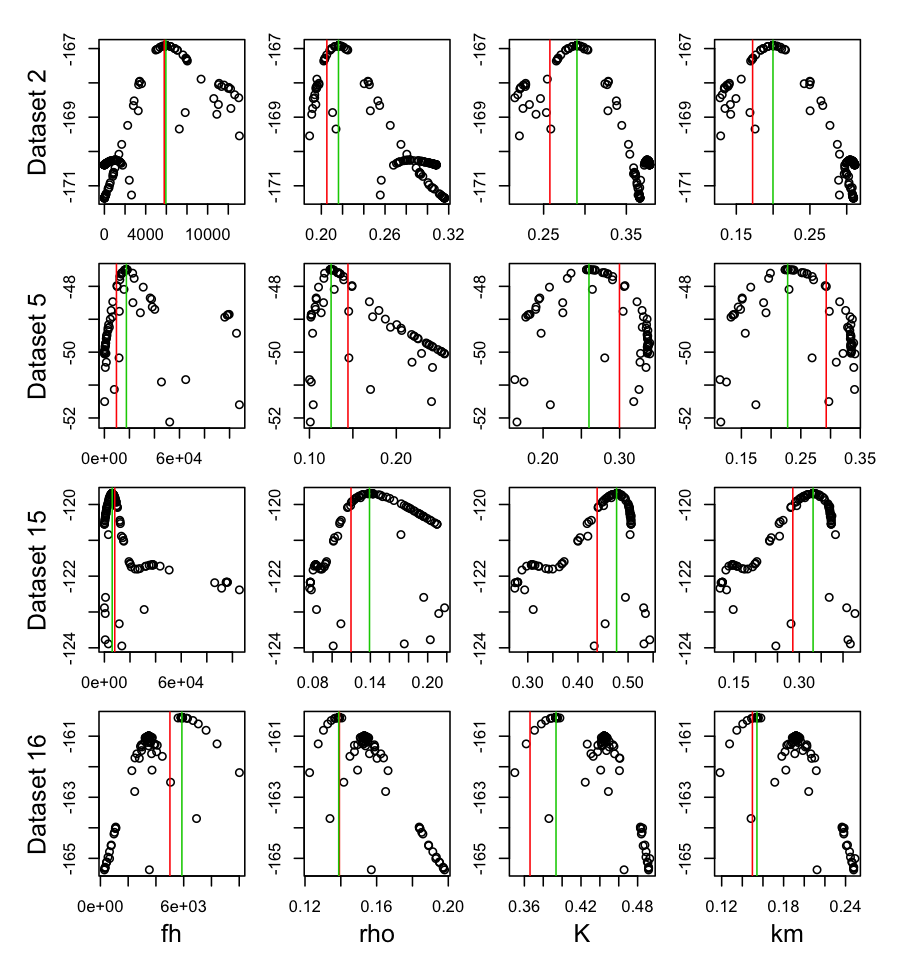
\includegraphics[width=\linewidth]{figure/lik-against-ests-1-1} \hfill{}

\caption[Plots of the likelihood against the parameter estimates for many of the datasets reveals a single likelihood peak, and most of the parameter estimates are quite close]{Plots of the likelihood against the parameter estimates for many of the datasets reveals a single likelihood peak, and most of the parameter estimates are quite close.}\label{fig:lik-against-ests-1}
\end{figure}


\end{knitrout}

On the other hand, Fig. \ref{fig:lik-against-ests-2} reveals that, for some of the datasets where the parameter estimates were further from the truth, the likelihood surface has multiple peaks.
In all of these cases, one of the likelihood peaks is centered around a high $f_h$ value.
In Fig. \ref{fig:lik-against-ests-2}, the likelihood is higher at this large $f_h$ peak, pulling all of the other parameter estimates away from their true values.

\begin{knitrout}\scriptsize
\definecolor{shadecolor}{rgb}{0.969, 0.969, 0.969}\color{fgcolor}\begin{figure}

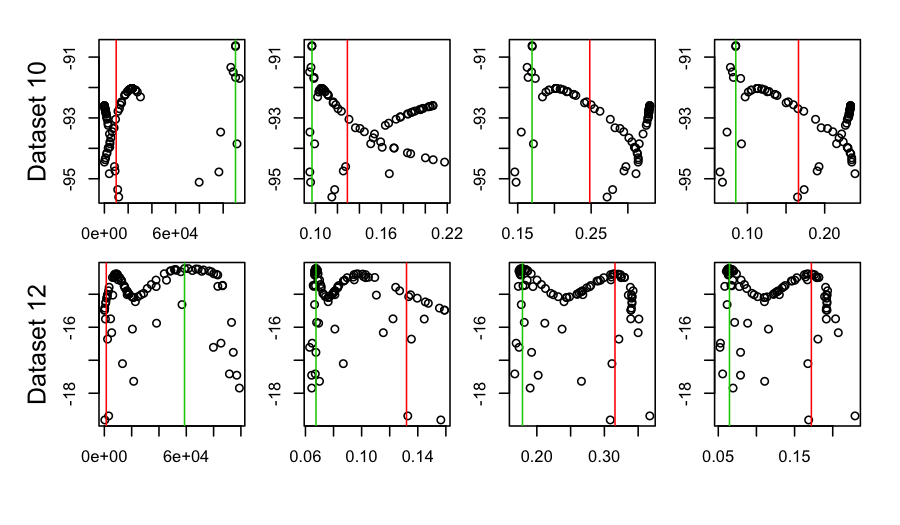
\includegraphics[width=\linewidth]{figure/lik-against-ests-2-1} \hfill{}

\caption[Plots of the likelihood against hte parameter estimates for some of the datasets reveals the existence of multiple likelihood peaks, one centered around a very high ]{Plots of the likelihood against hte parameter estimates for some of the datasets reveals the existence of multiple likelihood peaks, one centered around a very high $f_h$ value. When the likelihood is higher at this large $f_h$ peak, all of the other parameter estimates are pulled away from their true values.}\label{fig:lik-against-ests-2}
\end{figure}


\end{knitrout}

However, in Fig. \ref{fig:lik-against-ests-3}, you see cases where there are two peaks but the likelihood is higher at the peak with a low $f_h$ value.

\begin{knitrout}\scriptsize
\definecolor{shadecolor}{rgb}{0.969, 0.969, 0.969}\color{fgcolor}\begin{figure}

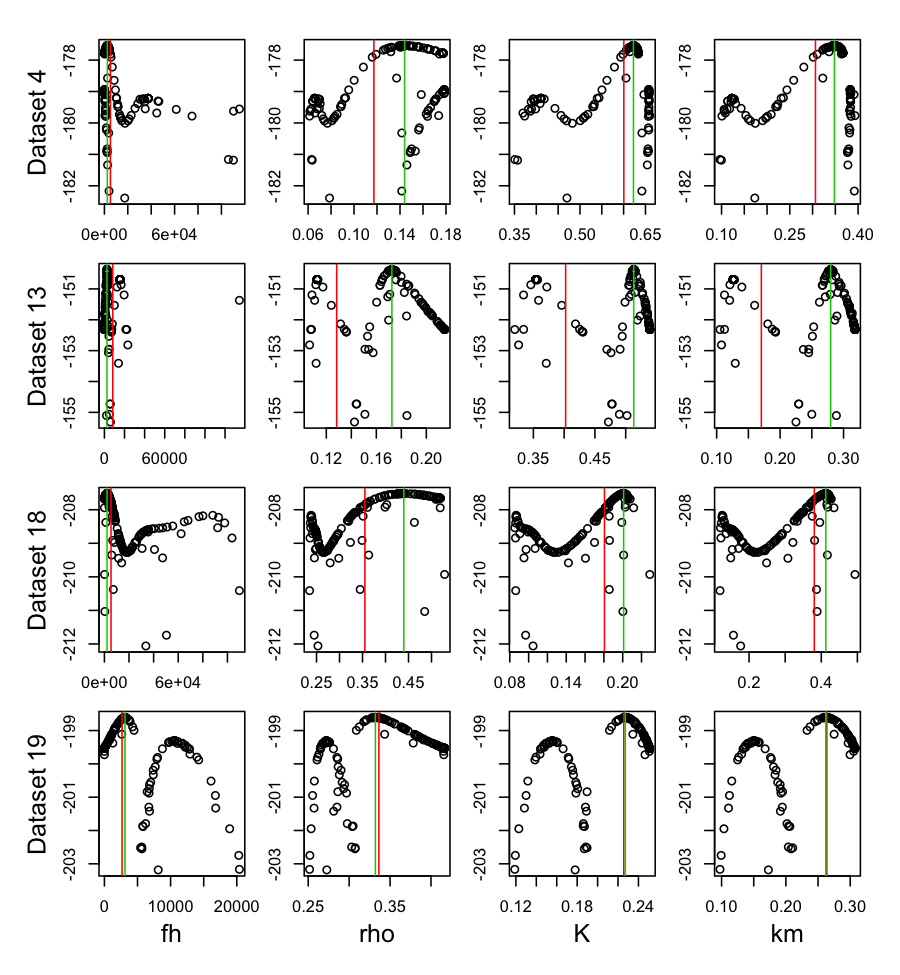
\includegraphics[width=\linewidth]{figure/lik-against-ests-3-1} \hfill{}

\caption[Plots of the likelihood against the parameter estimates for some of the datasets reveals the existence of multiple likelihood peaks]{Plots of the likelihood against the parameter estimates for some of the datasets reveals the existence of multiple likelihood peaks; in this case the likelihood is higher at the lower, more accurate, estimate.}\label{fig:lik-against-ests-3}
\end{figure}


\end{knitrout}

For still other datasets, the problem seems to be that the search algorithm got ``trapped'' at low values of $f_h$ (Fig. \ref{fig:lik-against-ests-4}).
It is possible that there was another peak in the likelihood surface at higher $f_h$ values that was never discovered by the fitting algorithm.

\begin{knitrout}\scriptsize
\definecolor{shadecolor}{rgb}{0.969, 0.969, 0.969}\color{fgcolor}\begin{figure}

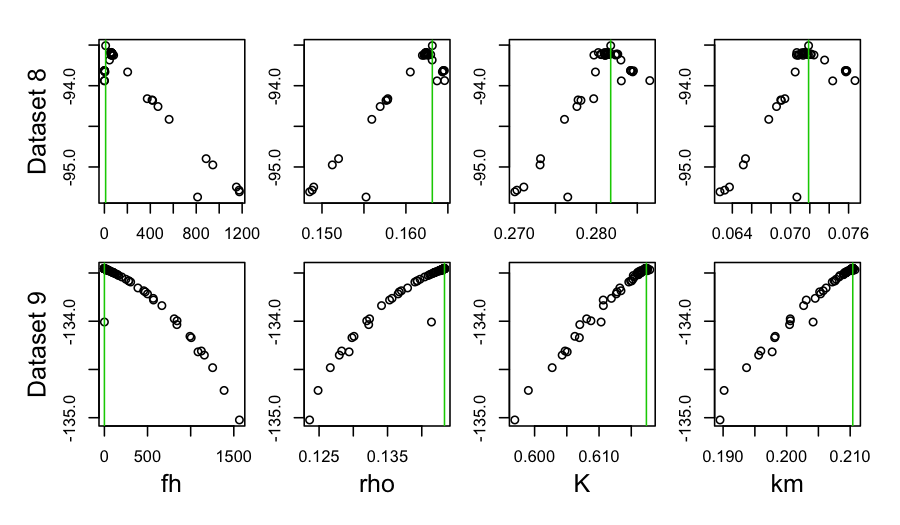
\includegraphics[width=\linewidth]{figure/lik-against-ests-4-1} \hfill{}

\caption[There were also datasets wherein the algorithm got stuck at low ]{There were also datasets wherein the algorithm got stuck at low $f_h$ values, never getting close to the truth.}\label{fig:lik-against-ests-4}
\end{figure}


\end{knitrout}

There were datasets that were simply hard to estimate, as evidenced by the fact that very few parameter sets had similar likelihoods (Fig. \ref{fig:lik-against-ests-5}).

\begin{knitrout}\scriptsize
\definecolor{shadecolor}{rgb}{0.969, 0.969, 0.969}\color{fgcolor}\begin{figure}

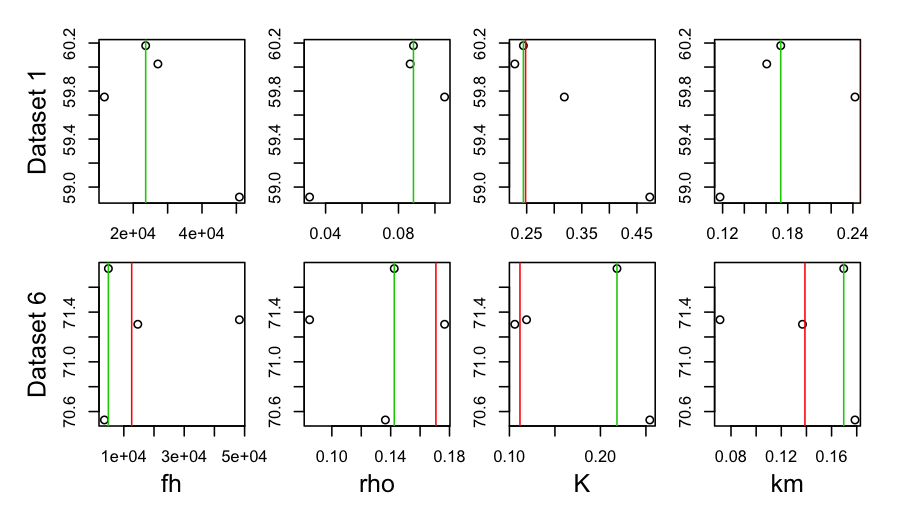
\includegraphics[width=\linewidth]{figure/lik-against-ests-5-1} \hfill{}

\caption[Some datasets were simply hard to estimate]{Some datasets were simply hard to estimate.}\label{fig:lik-against-ests-5}
\end{figure}


\end{knitrout}

\clearpage

However, if you compare the deterministic growth and reproduction trajectories at the true parameter values (red lines) to those trajectories at the best-fitting parameter set (black lines), you see that for all of the datasets, the best-fitting parameter set does a good job capturing the observed data (points).
You can see that, regardless of whether the parameter values were close to, or far from, the truth, the trajectories at the true and best-fitting parameters were always very close to one another.
The only things that you can conclude from looking at the fits is that datasets with very low reproduction are difficult to estimate, which makes sense - they are somewhat extreme.

\begin{knitrout}\scriptsize
\definecolor{shadecolor}{rgb}{0.969, 0.969, 0.969}\color{fgcolor}\begin{figure}

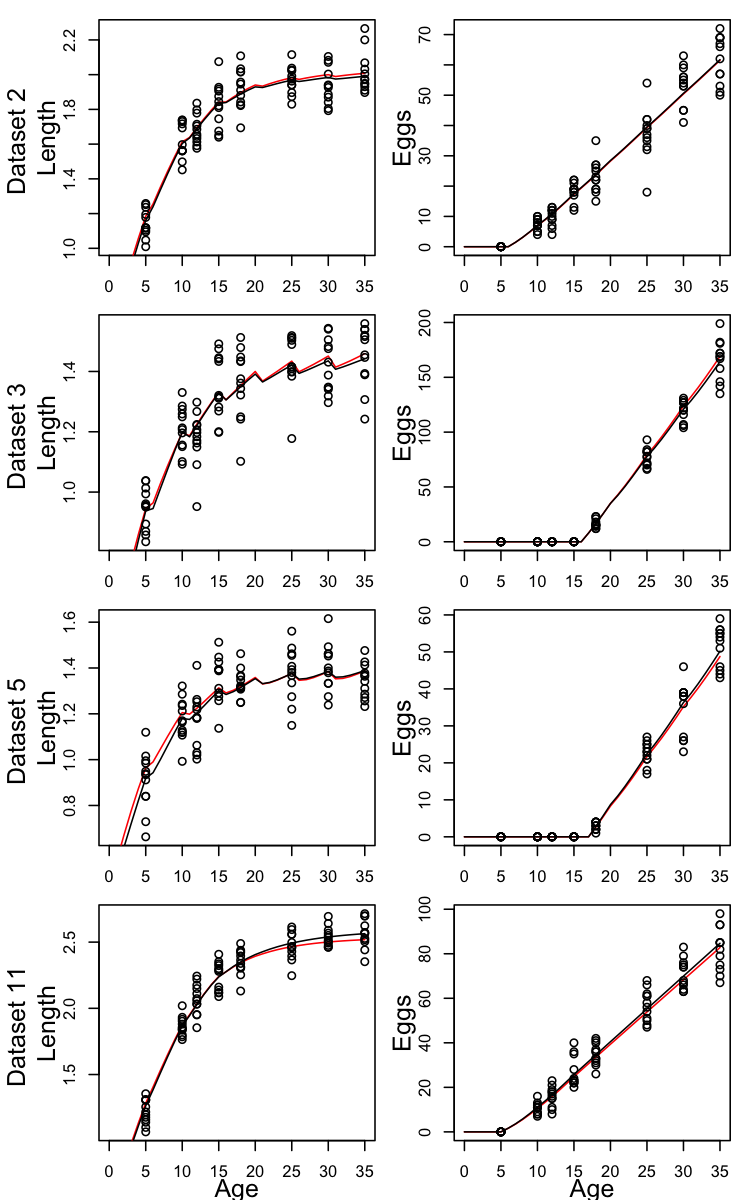
\includegraphics[width=0.6\textwidth]{figure/unnamed-chunk-1-1} \hfill{}

\caption[Plots of the raw observed length and egg data, along with the deterministic growth and reproduction trajectories at the true and best-fitting parameter sets]{Plots of the raw observed length and egg data, along with the deterministic growth and reproduction trajectories at the true and best-fitting parameter sets. Here we show those trajectories for parameter sets that were close to the truth.}\label{fig:unnamed-chunk-1}
\end{figure}


\end{knitrout}

\begin{knitrout}\scriptsize
\definecolor{shadecolor}{rgb}{0.969, 0.969, 0.969}\color{fgcolor}\begin{figure}

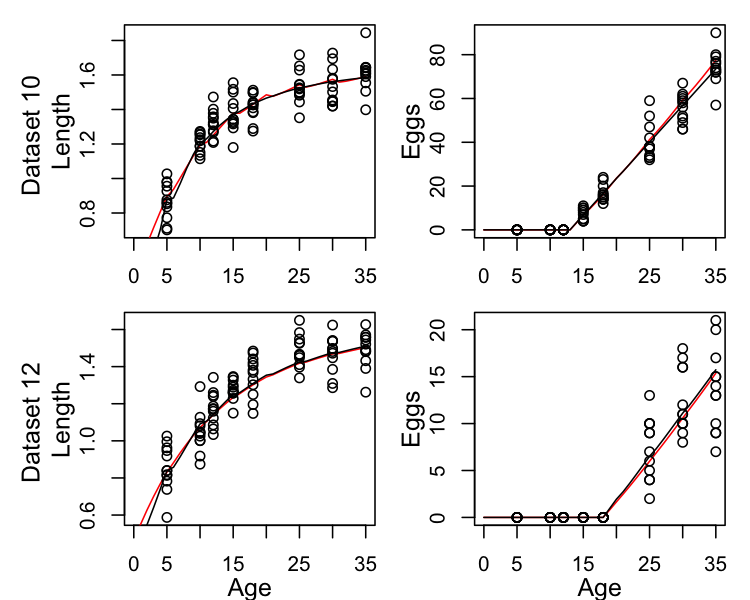
\includegraphics[width=0.6\textwidth]{figure/unnamed-chunk-2-1} \hfill{}

\caption[Plots of the raw observed length and egg data, along with the deterministic growth and reproduction trajectories at the true and best-fitting parameter sets]{Plots of the raw observed length and egg data, along with the deterministic growth and reproduction trajectories at the true and best-fitting parameter sets. Here are the trajectories for datasets that yielded two likelihood peaks and the best-fitting parameter set was far from the truth.}\label{fig:unnamed-chunk-2}
\end{figure}


\end{knitrout}

\begin{knitrout}\scriptsize
\definecolor{shadecolor}{rgb}{0.969, 0.969, 0.969}\color{fgcolor}\begin{figure}

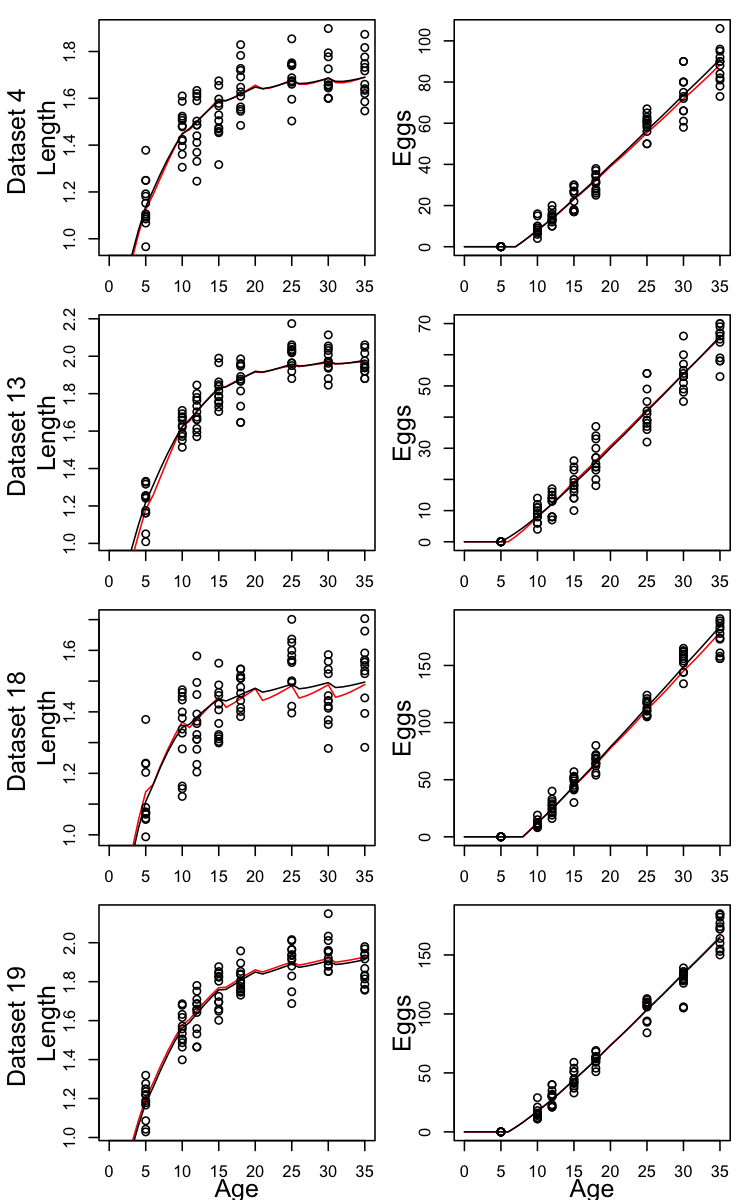
\includegraphics[width=0.6\textwidth]{figure/unnamed-chunk-3-1} \hfill{}

\caption[Plots of the raw observed length and egg data, along with the deterministic growth and reproduction trajectories at the true and best-fitting parameter sets]{Plots of the raw observed length and egg data, along with the deterministic growth and reproduction trajectories at the true and best-fitting parameter sets. Here are the trajectories for datasets that yielded two likelihood peaks and the best-fitting parameter set was closer to the truth.}\label{fig:unnamed-chunk-3}
\end{figure}


\end{knitrout}

\begin{knitrout}\scriptsize
\definecolor{shadecolor}{rgb}{0.969, 0.969, 0.969}\color{fgcolor}\begin{figure}

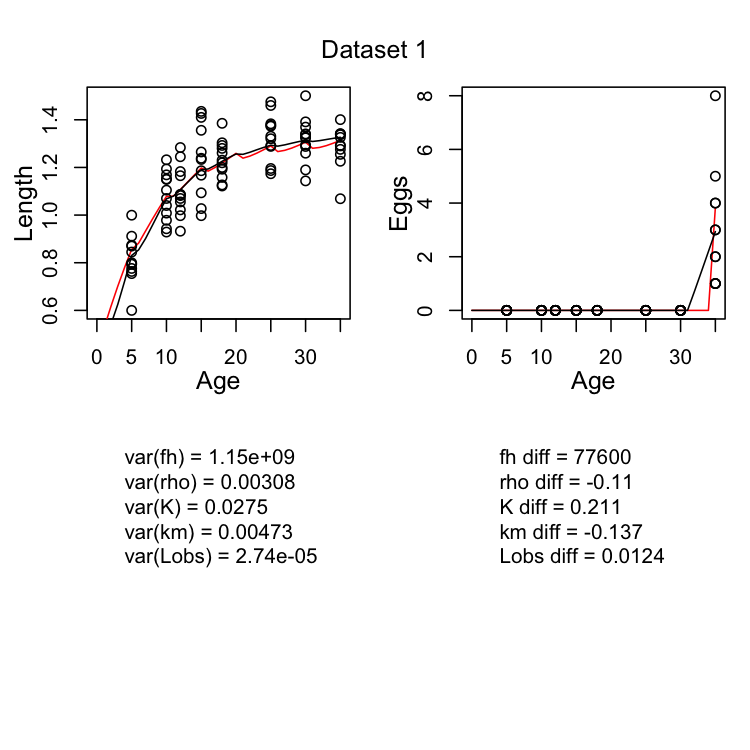
\includegraphics[width=0.6\textwidth]{figure/unnamed-chunk-4-1} \hfill{}

\caption[Plots of the raw observed length and egg data, along with the deterministic growth and reproduction trajectories at the true and best-fitting parameter sets]{Plots of the raw observed length and egg data, along with the deterministic growth and reproduction trajectories at the true and best-fitting parameter sets. Here are the trajectories when the parameter estimates got stuck at low $f_h$ values (8,9) or where the parameters were simply hard to estimate (1,6).}\label{fig:unnamed-chunk-4}
\end{figure}


\end{knitrout}
\clearpage

Overall, I think the message from these simulation-recovery experiments is highly encouraging.
I think, at a maximum, that it may be necessary to carry out profile likelihood calculations for $f_h$ and possibly also $v$ (just to ensure that changing the value of $v$ has no effect).
But these simulations do lend credence to our ability to estimate $\rho$, $\kappa$, and $k_m$, so long as the other parameters related to feeding, length-biomass conversion, and the cost of reproduction are known.

\end{document}
